\documentclass[border=6pt]{standalone}
% Compile with xelatex (build_overview.sh). All text is Arial; at the printed size
% (300 dpi TIFF) \footnotesize (8.1 TeX pt, below) is the smallest size used.
\usepackage{fontspec}
\setmainfont{Arial}\setsansfont{Arial}
\renewcommand{\familydefault}{\sfdefault}
% \footnotesize is 8 TeX pt = 7.97 PostScript pt; use 8.1 TeX pt (8.07 PostScript pt) so no text is below 8 pt.
\renewcommand{\footnotesize}{\fontsize{8.1}{9.7}\selectfont}
\usepackage{tikz}
\usetikzlibrary{positioning,arrows.meta,fit,backgrounds}
\definecolor{ink}{HTML}{0B0B0B}\definecolor{ink2}{HTML}{52514E}
\definecolor{fw}{HTML}{CDE2FB}\definecolor{fwb}{HTML}{2A78D6}
\definecolor{ev}{HTML}{F3F2EE}\definecolor{evb}{HTML}{898781}
\definecolor{st}{HTML}{FDE3D7}\definecolor{stb}{HTML}{EB6834}
\begin{document}
\footnotesize
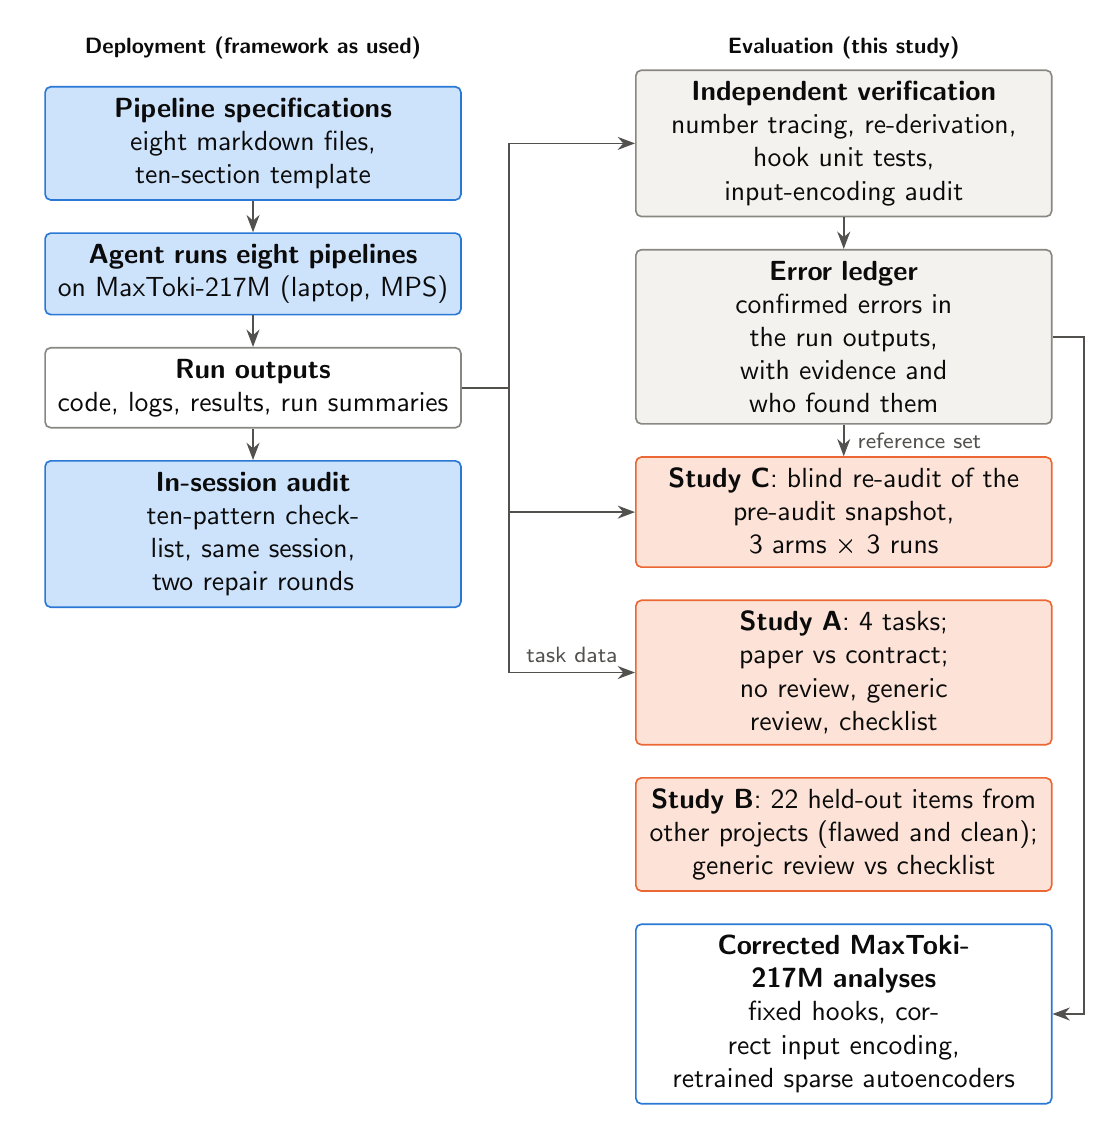
\begin{tikzpicture}[
  box/.style={draw=#1, line width=0.6pt, rounded corners=2pt, align=center, text width=5.0cm, inner sep=4pt, text=ink},
  arr/.style={-{Stealth[length=2.2mm]}, line width=0.6pt, draw=ink2},
  node distance=4mm]
% ---------------- deployment column
\node[box=fwb, fill=fw] (spec) {\textbf{Pipeline specifications}\\eight markdown files, ten-section template};
\node[box=fwb, fill=fw, below=of spec] (run) {\textbf{Agent runs eight pipelines}\\on MaxToki-217M (laptop, MPS)};
\node[box=evb, fill=white, below=of run] (out) {\textbf{Run outputs}\\code, logs, results, run summaries};
\node[box=fwb, fill=fw, below=of out] (audit) {\textbf{In-session audit}\\ten-pattern checklist, same session,\\two repair rounds};
\draw[arr] (spec) -- (run); \draw[arr] (run) -- (out); \draw[arr] (out) -- (audit);
\begin{scope}[on background layer]
\node[fit=(spec)(audit), inner sep=6pt, draw=none, fill=none, label={[name=deplab, text=ink, font=\footnotesize\bfseries]above:Deployment (framework as used)}] (dep) {};
\end{scope}
% ---------------- evaluation column
\node[box=evb, fill=ev, right=22mm of spec] (ver) {\textbf{Independent verification}\\number tracing, re-derivation,\\hook unit tests, input-encoding audit};
\node[box=evb, fill=ev, below=of ver] (led) {\textbf{Error ledger}\\confirmed errors in the run outputs,\\with evidence and who found them};
\node[box=stb, fill=st, below=of led] (sc) {\textbf{Study C}: blind re-audit of the\\pre-audit snapshot, 3 arms \texttimes{} 3 runs};
\node[box=stb, fill=st, below=of sc] (sa) {\textbf{Study A}: 4 tasks; paper vs contract;\\no review, generic review, checklist};
\node[box=stb, fill=st, below=of sa] (sb) {\textbf{Study B}: 22 held-out items from\\other projects (flawed and clean);\\generic review vs checklist};
\node[box=fwb, fill=white, below=of sb] (cs) {\textbf{Corrected MaxToki-217M analyses}\\fixed hooks, correct input encoding,\\retrained sparse autoencoders};
\draw[arr] (ver) -- (led); \draw[arr] (led) -- node[right, xshift=0.5mm, text=ink2, font=\footnotesize]{reference set} (sc);
\draw[arr] (out.east) -- ++(6mm,0) |- (ver.west);
\draw[arr] (out.east) -- ++(6mm,0) |- (sc.west);
\draw[arr] (out.east) -- ++(6mm,0) |- node[pos=0.75, above, text=ink2, font=\footnotesize]{task data} (sa.west);
\draw[arr] (led.east) -- ++(4mm,0) |- (cs.east);
\node[anchor=base, text=ink, font=\footnotesize\bfseries] at (ver.north |- deplab.base) {Evaluation (this study)};
\end{tikzpicture}
\end{document}
